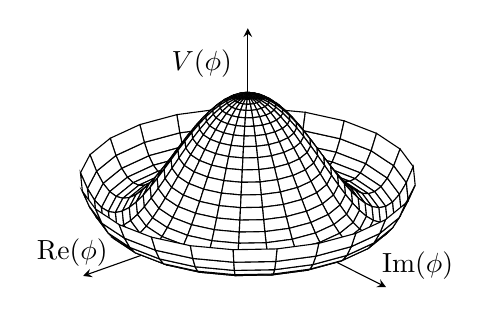
\begin{tikzpicture}
  \begin{axis}[
      axis lines=center,
      view={140}{25},
      axis equal,
      domain=0:360,
      y domain=0:1.25,
      xmax=1.6,ymax=1.6,zmin=0,zmax=1.3,
      x label style={at={(axis description cs:0.18,0.33)},anchor=north},
      y label style={at={(axis description cs:0.82,0.30)},anchor=north},
      z label style={at={(axis description cs:0.42,0.75)},anchor=north},
      xlabel = $\mathrm{Re}(\phi)$,
      ylabel=$\mathrm{Im}(\phi)$,
      zlabel=$V(\phi)$,
      ticks=none,
      clip bounding box=upper bound
    ]

    \addplot3 [surf, shader=flat, draw=black, fill=white, z buffer=sort] ({sin(x)*y}, {cos(x)*y}, {(y^2-1)^2});
  \end{axis}
\end{tikzpicture}